\begin{figure}
    \begin{center}
    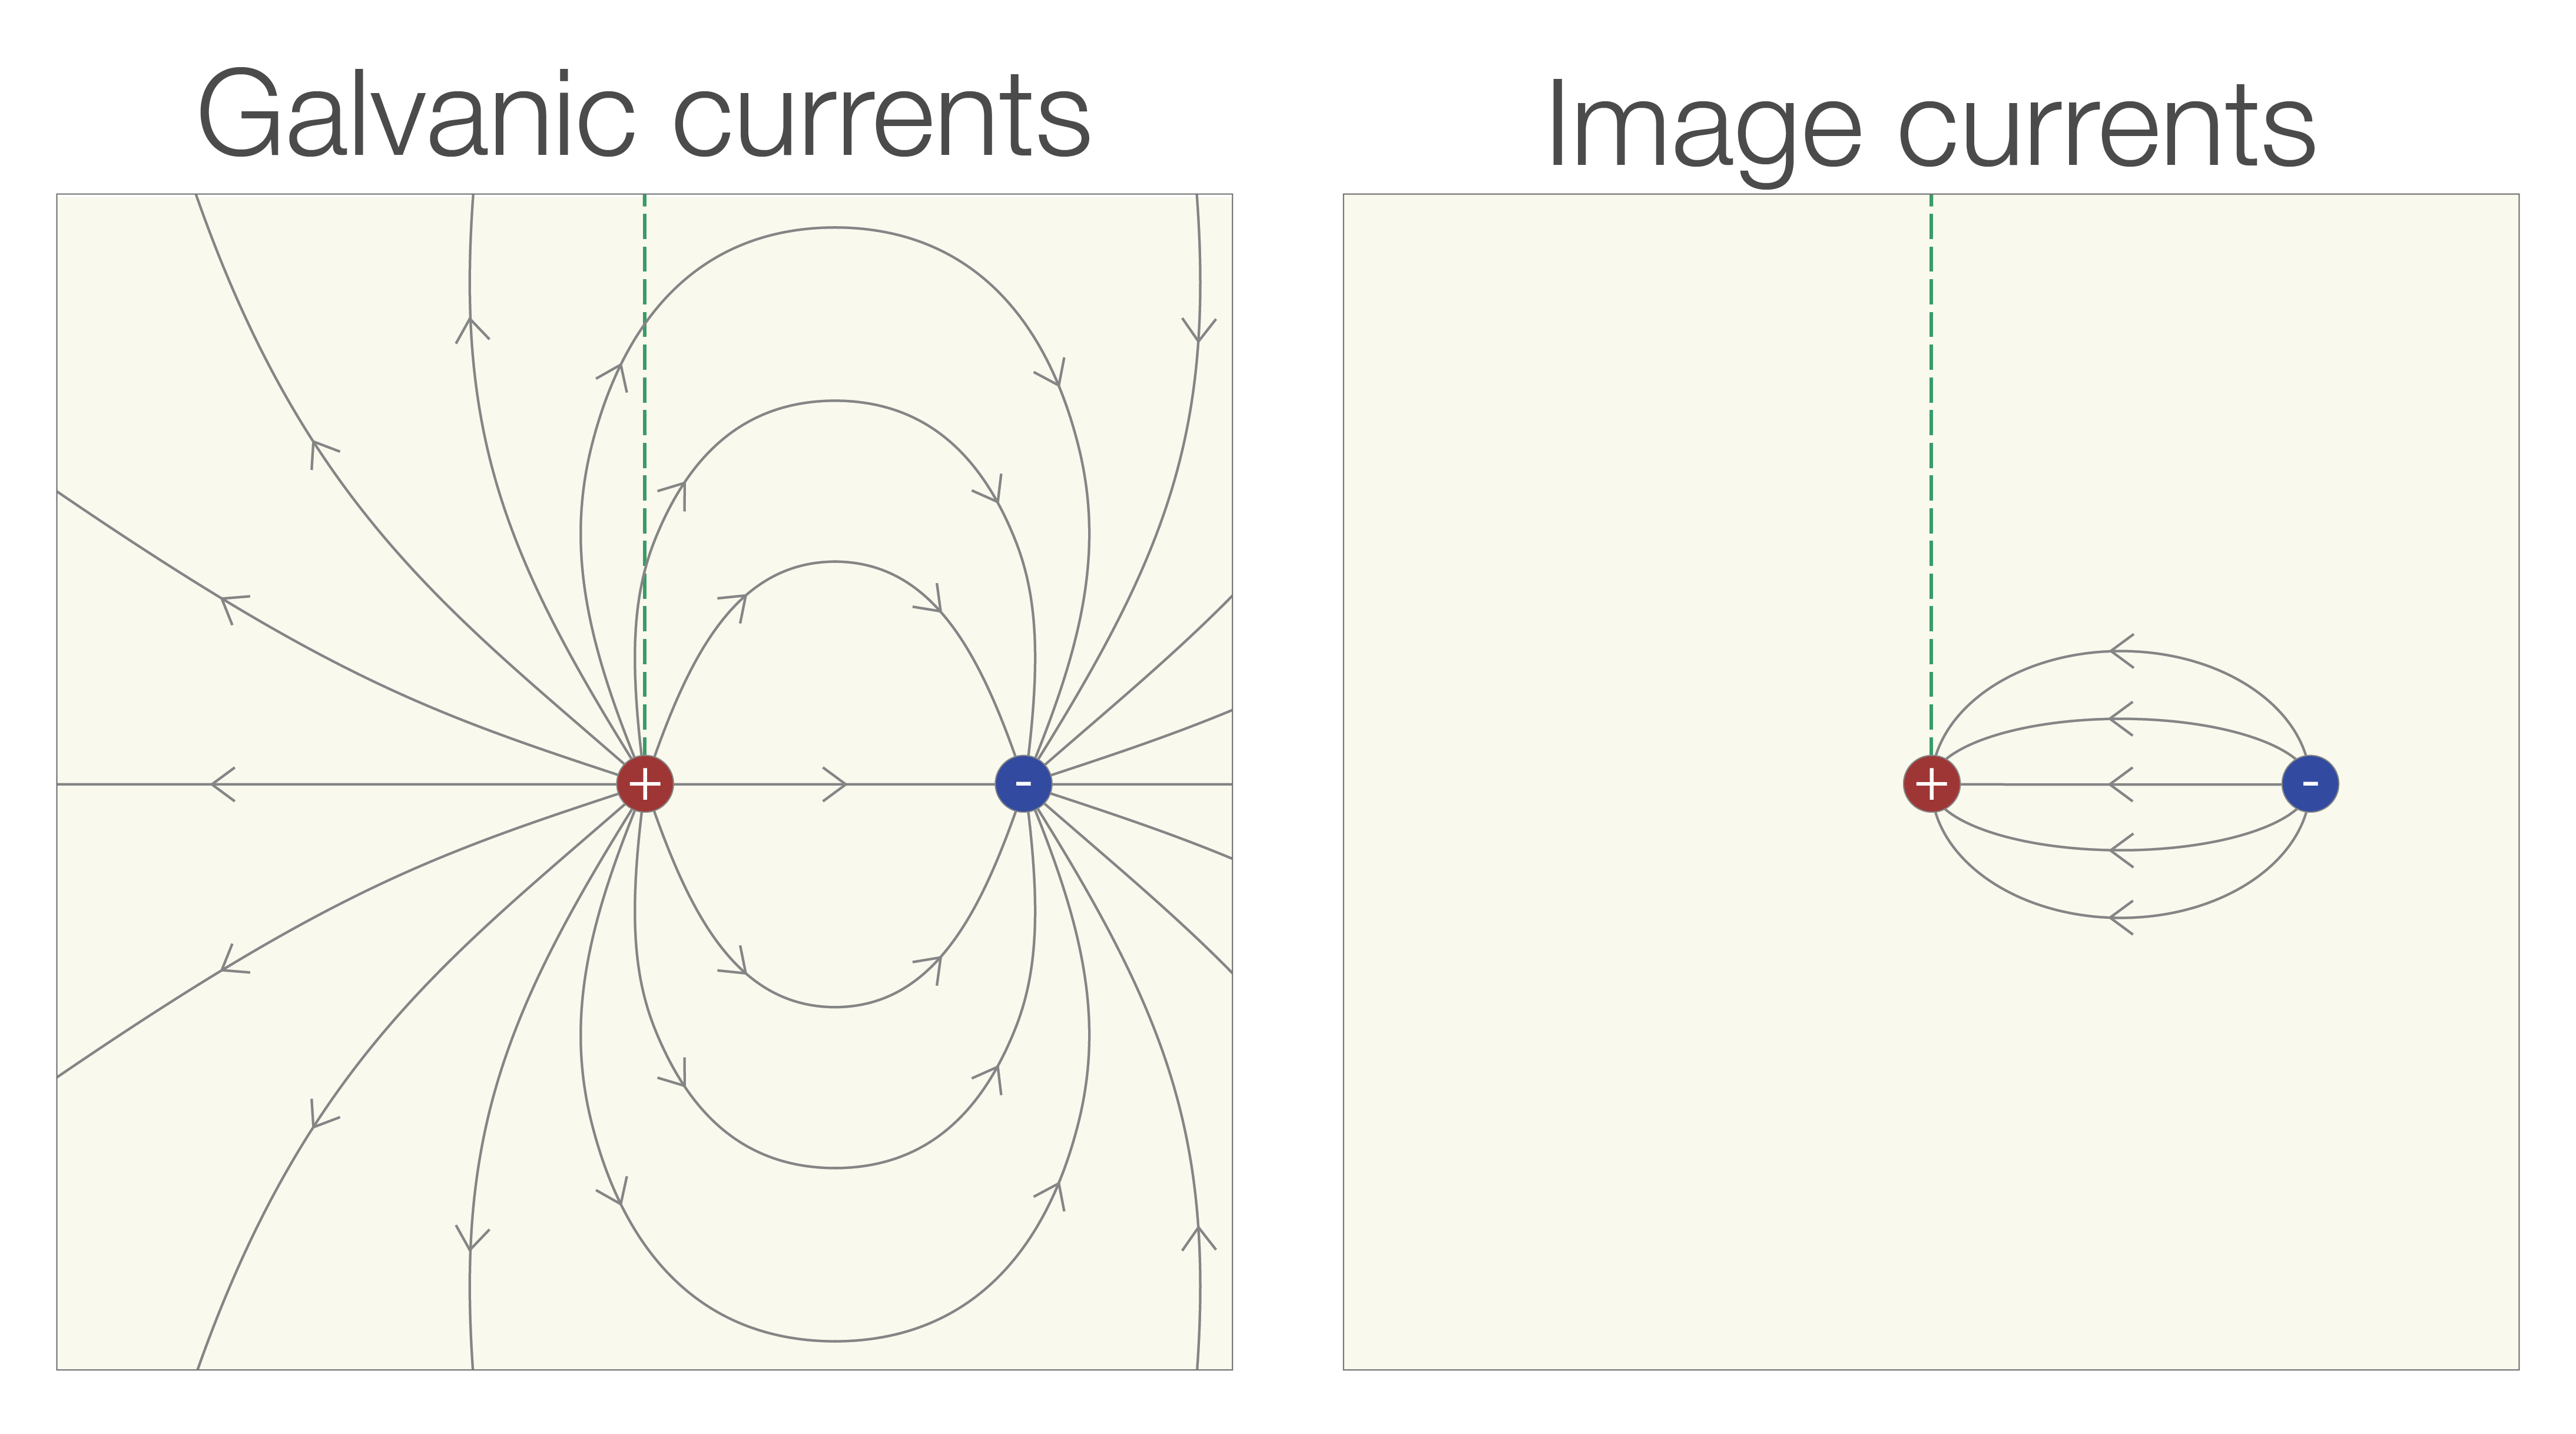
\includegraphics[width=0.75\textwidth]{figures/current-systems-sketch.png}
    \end{center}
\caption{
    Sketch of the plan-view geometry of the early-time galvanic currents (left) and image currents (right) in a time-domain EM experiment over a half-space.
    Through time, both current systems diffuse downwards and outwards as they decay.
    The wire follows a straight line between the negative and positive electrodes. The green dashed line shows where we are measuring the
    radial electric field data. Prior to shut-off, current in the wire flows from
    the negative to the positive electrode. In the earth, the galvanic currents are dipolar in nature and flow
    from the positive to the negative electrode. Along the survey-line, the radial component of the galvanic currents always points outwards.
    Immediately after shut-off, image currents are induced in the earth. They are oriented in the same direction as the original current in the wire
    and are directed away from the negative electrode towards the positive. Along the survey-line, the radial component of the image currents is always pointed inwards.
}
\label{fig:current-systems-sketch}
\end{figure}



